\documentclass[14pt]{article}

\includeonly{chapter02,chapter03}

\usepackage{amssymb}
\usepackage{amsthm}
\usepackage{mathtools}
\usepackage{tikz}
\usepackage{wasysym}
\usetikzlibrary{fit}
\usetikzlibrary{positioning}
\usetikzlibrary{shapes}

\newcommand{\exercise}[1]{\subsection*{Exercise #1}}
\newcommand{\Hom}[1]{\mathrm{Hom}_{\mathbf{#1}}}
\newcommand{\id}[1]{\mathrm{id}_{#1}}
\newcommand{\llangle}{\langle\!\langle\,}
\newcommand{\rrangle}{\,\rangle\!\rangle}

\newtheorem*{thm}{Theorem}

\let\oldemptyset\emptyset{}
\let\emptyset\varnothing{}

\tikzset{aspect/.style={draw=black,->,>=stealth,shorten >=7pt,shorten <=7pt,auto}}
\tikzset{type/.style={rectangle,draw=black,fill=white,thick}}
\tikzset{aspects/.style={every edge/.style=aspect}}
\tikzset{types/.style={row sep=4em, column sep=4em, every node/.style=type}}

\begin{document}
\section*{Chapter 2}


\exercise{2.1.1.2}
$\mathcal{P}(A) = \emptyset, \{1\}, \{2\}, \{3\}, \{1,2\}, \{1,3\}, \{2,3\}, \{1,2,3\}$


\exercise{2.1.1.3}
\paragraph{a.}
A function $PR \to RG$.
\paragraph{b.}
Yes, there are probably many many-to-one connection points.


\exercise{2.1.2.5}
\paragraph{a.}
$2 \mapsto 4$
\paragraph{b.}
$0 \mapsto 0$
\paragraph{c.}
Not applicable; $-2 \not\in \mathbb{N}$.
\paragraph{d.}
$5 \mapsto 25$
\paragraph{e.}
The symbol $\to$ associates the domain and codomain, while $\mapsto$
associates a particular member of the domain to a particular member of
the codomain.


\exercise{2.1.2.6}
$\operatorname{im}(f) = \{y_1, y_2, y_4\}$


\exercise{2.1.2.8}
$f(A) = \{0,1,4,9\}$


\exercise{2.1.2.10}
$f \circ x \colon \{\smiley\} \to Y$ and $\smiley \mapsto f(x)$.


\exercise{2.1.2.12}
\paragraph{a.}
$2^5 = 32$
\paragraph{b.}
$5^2 = 25$


\exercise{2.1.2.13}
\paragraph{a.}
Take $A := \{\smiley\}$.  (e.g. $A := $
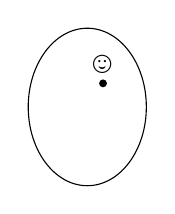
\begin{tikzpicture}
  \draw (0,0) ellipse [x radius = 0.75, y radius = 1];
  \fill (0.2,0.3) circle [radius=0.05] node[anchor=south]{\smiley};
\end{tikzpicture}
, $X := $
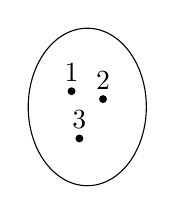
\begin{tikzpicture}
  \draw (0,0) ellipse [x radius = 0.75, y radius = 1];
  \fill (-0.2,0.2) circle [radius=0.05] node[anchor=south]{1};
  \fill (0.2,0.1) circle [radius=0.05] node[anchor=south]{2};
  \fill (-0.1,-0.4) circle [radius=0.05] node[anchor=south]{3};
\end{tikzpicture}
)
\paragraph{b.}
$B := \emptyset$.  (e.g. $B := $
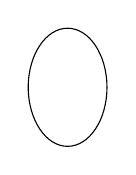
\begin{tikzpicture}
    \draw (0,0) ellipse [x radius = 0.50, y radius = 0.75];
\end{tikzpicture}
)


\exercise{2.1.2.17}
\paragraph{a.}
$n!\,$
\paragraph{b.}
Yes, $0! = 1$.


\exercise{2.1.2.19}
No.


\exercise{2.1.2.20}
Take $A := \{\smiley\}$.


\exercise{2.1.2.22}
\paragraph{a.}
$f(4) = c$
\paragraph{b.}
$f = \left(1,4,9,16,25,36,49\right)$


\exercise{2.1.2.24}
\paragraph{a.}
3
\paragraph{b.}
4
\paragraph{c.}
$\lvert\mathbb{N}\rvert \geqslant \infty$
\paragraph{d.}
$\lvert\lbrace n \in \mathbb{N} \mid n \leqslant 5 \rbrace \rvert =
 \lvert\lbrace 0,1,2,3,4,5\rbrace\rvert = 6$


\exercise{2.3.2.7}
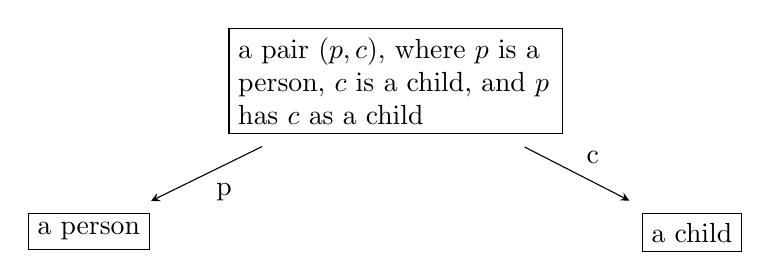
\begin{tikzpicture}[->,>=stealth,shorten >=10pt,shorten <=10pt,auto]
  \node [shape=rectangle,draw,text width=4cm] (R)
  {
    a pair $(p,c)$, where $p$ is a person, $c$ is a child, and $p$ has
    $c$ as a child
  };
  \node [shape=rectangle,draw,below left=of R] (P) {a person};
  \node [shape=rectangle,draw,below right=of R] (C) {a child};

  \path (R) edge node {p} (P)
            edge node {c} (C);
\end{tikzpicture}


%%% Local Variables:
%%% mode: latex
%%% TeX-master: "exercises"
%%% End:

\section*{Chapter 3}


\exercise{3.1.1.4}
$4 \times 3 = 12$ elements


\exercise{3.1.1.8}
\paragraph{a.}
\begin{align*}
  (a,b,c)\mapsto(a+b,c); (x,y)\mapsto xy
  &= (a,b,c)\mapsto ac+bc \\
  (a,b,c)\mapsto(a\cdot b,a\cdot c); (x,y)\mapsto x+y
  &= (a,b,c)\mapsto ab+ac
\end{align*}
does not commute
\paragraph{b.}
\begin{align*}
  x\mapsto(x,0); (a,b)\mapsto(a\cdot b) &= x\mapsto 0 \\
  id_\mathbb{Z} &= x\mapsto x
\end{align*}
does not commute
\paragraph{c.}
\begin{align*}
  x\mapsto(x,1); (a,b)\mapsto(a\cdot b) &= x\mapsto x \\
  id_\mathbb{Z} &= x\mapsto x
\end{align*}
commutes


\exercise{3.1.1.13}
Here is a relationship between them:
\begin{equation*}
  \Hom{Set}(A,X) \times \Hom{Set}(A,Y) \cong \Hom{Set}(A,X \times Y)\,.
\end{equation*}


\exercise{3.1.1.14}
\paragraph{a.}
\begin{equation*}
  s \colon X \times Y \to Y \times X \coloneqq
  \left\langle \pi_2 , \pi_1 \right\rangle \,.
\end{equation*}
\paragraph{b.}
\begin{thm}
  The swap map $s$ above is an isomorphism.
\end{thm}
\begin{proof}
  Note that
  \begin{align*}
    \left\langle p_2 , p_1 \right\rangle \cdot
    \left\langle \pi_2 , \pi_1 \right\rangle \cdot
    p_2
    &= \left\langle p_2 , p_1 \right\rangle \cdot
      \pi_1 \\
    &= p_2
  \end{align*}
  and similarly with $p_1$ and $\pi_2$.

  The universal property for products with
  $p_1$ and $p_2$ implies that
  \begin{equation*}
    \left\langle p_2 , p_1 \right\rangle \cdot
    \left\langle \pi_2 , \pi_1 \right\rangle =
    \id{Y \times X}
  \end{equation*}
  by unicity.

  The other direction is similar.
\end{proof}


\exercise{3.1.2.4}
Yes, it is conceivable that
$\lceil\mathrm{a\ phone}\rceil =
\lceil\mathrm{a\ cell\ phone}\rceil \sqcup
\lceil\mathrm{a\ landline\ phone}\rceil$.


\exercise{3.1.2.9}
\paragraph{a.}
$f(n) = \lvert n \rvert$.
\paragraph{b.}
$A = \mathbb{N},
X = \{\,n \in \mathbb{Z} \,\vert\, n \geqslant 0\,\},
Y = \{\,n \in \mathbb{Z} \,\vert\, n < 0\,\},
X \sqcup Y \cong \mathbb{Z}$.


\exercise{3.1.2.12}
$\Hom{Set}(X,A) \times \Hom{Set}(Y,A) \cong \Hom{Set}(X \sqcup Y,A)$


\exercise{3.1.2.15}
Let $c,d$ be objects.  Then
\begin{equation*}
  \llangle c \sqcup d \rrangle \coloneqq
  \textrm{``either $\llangle c \rrangle$, labled as such, or $\llangle
    d \rrangle$, labled as such.''}
\end{equation*}

The inclusions $c \rightarrow c \sqcup d \leftarrow d$ may be read
``is, when appropriately labled.''


\begin{tikzpicture}
  \matrix [types]
  {
    \node (W) {a wav file}; &
    \node (A) {an audio file}; &
    \node (M) {an mp3 file}; \\
  };
  \path [aspects]
  (W) edge node [above] {is, with the ``.wav'' extension} (A)
  (M) edge node [above] {is, with the ``.mp3'' extension} (A);
\end{tikzpicture}


%%% Local Variables:
%%% mode: latex
%%% TeX-master: "exercises"
%%% End:

\end{document}
